\documentclass[presentation]{beamer}
\mode<presentation>{\usetheme{AMSBolognaFCrev}}

\usepackage[utf8]{inputenc}
\usepackage[T1]{fontenc}
\usepackage{booktabs}
\usepackage{array}
\usepackage{tabularx}
\usepackage{tikz}
\usepackage[ddmmyyyy]{datetime}
\usepackage[export]{adjustbox}
\usetikzlibrary{arrows.meta,positioning,shapes.geometric,fit,calc}

\renewcommand{\dateseparator}{/}
\newcommand{\sectiontitleframe}[1]{
\begin{frame}[plain,c]
\begin{center}
{\usebeamerfont{title}\usebeamercolor[fg]{title}#1}
\end{center}
\end{frame}
}

\tikzset{
    privacybox/.style={draw, rounded corners, align=center, font=\scriptsize,
        minimum height=0.72cm, text width=2.25cm},
    smallprivacybox/.style={draw, rounded corners, align=center, font=\tiny,
        minimum height=0.55cm, text width=1.65cm},
    privacyarrow/.style={-{Stealth[length=2mm]}, thick}
}

\title[Lesson 8]{Healthcare Privacy and Data Protection}
\institute[Data Privacy and Security]{Healthcare Data Privacy and Security}
\author[\sspeaker{G. Pisano}]{\speaker{Giuseppe Pisano} \\\href{mailto:g.pisano@unibo.it}{g.pisano@unibo.it}}
\date[August, 2026]{August, 2026}
%
\titlegraphic{
\begin{center}
    
\includegraphics[width=0.35\textwidth, valign=c]{logos/intestazione.png}
    
\includegraphics[width=0.16\textwidth, valign=c]{logos/unibo_logo_2.png}
    
\includegraphics[width=0.11\textwidth, valign=c]{logos/makeni_logo_2.png}
    
\includegraphics[width=0.20\textwidth, valign=c]{logos/cuamm_logo_png.png}
\end{center}
\centering
\tiny{S.K.I.L.L.E.D --- AID013244/04/2\\Strategic Knowledge and Inclusive Lifelong Learning in the health sector for youth Employability and Development}
}

\newcommand{\scenario}{St. Isidore Hospital}
\newcommand{\takeawaysframe}[2]{
\begin{frame}[c]{Recap: \insertsection}
\begin{block}{Takeaways}
#1
\end{block}
\begin{exampleblock}{In \scenario}
#2
\end{exampleblock}
\end{frame}
}

\begin{document}

\setbeamertemplate{frametitle}
{
    \nointerlineskip
    \begin{beamercolorbox}[sep=0.3cm,ht=2.2em,wd=\paperwidth]{frametitle}
        \vbox{}\vskip-2ex%
        \strut\insertframetitle\hfill\raisebox{-0.2\height}{
\includegraphics[width=2cm]{logos/cuamm_logo_png.png}}\strut
        \vskip-0.8ex%
    \end{beamercolorbox}
}

\begin{frame}[allowframebreaks]
\titlepage
\end{frame}

\begin{frame}[c,allowframebreaks]{Roadmap}
\tableofcontents[hideallsubsections]
\end{frame}

\begin{frame}[c]{How This Lesson Progresses}
\begin{block}{Learning path}
We move from the idea of \textbf{privacy} as private life, to \textbf{data protection} as control
over information, and finally to concrete duties for healthcare systems that process patient data.
\end{block}

\begin{exampleblock}{Hospital storyline}
\scenario{} wants to use electronic health records, laboratory systems, telemedicine, research
datasets, and AI triage support. Each system may be useful, but each changes who can see, copy,
combine, or infer sensitive information about patients.
\end{exampleblock}
\end{frame}

\begin{frame}[c]{GDPR as an Example, Not the Whole Map}
\begin{block}{Position of this lesson}
The GDPR is used here as a detailed example of modern data protection law. It is influential
globally, but it is not the only model: HIPAA, CCPA, POPIA, APEC privacy approaches, African and
national health-data frameworks, and professional ethics also matter.
\end{block}

\begin{exampleblock}{Why it is useful}
GDPR makes many core ideas explicit: personal data, processing, controller, processor, legal basis,
purpose limitation, minimization, rights, accountability, data protection by design, breach duties,
and supervision.
\end{exampleblock}
\end{frame}

\section{From Privacy to Data Protection}
\sectiontitleframe{From Privacy to Data Protection}

\begin{frame}[c]{Section Context: From Privacy to Data Protection}
\begin{block}{What we are talking about}
Privacy began as protection against unwanted intrusion into private life. In digital healthcare, the
problem expands: patients may not only be watched; their data can be stored, linked, reused,
exported, profiled, and breached.
\end{block}

\begin{exampleblock}{Hospital lens}
A doctor overhearing private symptoms in a corridor is a privacy problem. A database exporting lab
results to an insurer without a valid reason is a data protection problem.
\end{exampleblock}
\end{frame}

\begin{frame}[c]{Origins: The Right to Be Let Alone}
\begin{block}{Classical idea}
Modern privacy discourse is often traced to Warren and Brandeis and the idea of a right to be
``let alone'' \cite{warren_brandeis}. This model protects private life, habits, writings, images,
family life, and reputation from unjustified exposure.
\end{block}

\begin{exampleblock}{Running example}
If a hospital employee shares a celebrity patient's ward photo with a newspaper, the harm is not
only security failure. It is an invasion of private life and dignity.
\end{exampleblock}
\end{frame}

\begin{frame}[c]{Privacy as a Fundamental Right}
\begin{block}{Human-rights dimension}
Privacy becomes more than a private-law claim. It protects autonomy, family life, correspondence,
home, dignity, and democratic freedom. International and European instruments frame it as a right
against arbitrary interference \cite{udhr,echr}.
\end{block}

\begin{exampleblock}{Running example}
A public hospital is part of the state. If it centralizes patient records, the issue is not only
employee curiosity; public power must also be constrained by law, necessity, and safeguards.
\end{exampleblock}
\end{frame}

\begin{frame}[c]{Decision Privacy and Information Privacy}
\begin{block}{Two faces}
\textbf{Decision privacy} protects autonomy in intimate and family choices. \textbf{Information
privacy} protects control over the circulation of information about those choices.
\end{block}

\begin{exampleblock}{Running example}
A patient's decision to seek reproductive care involves decision privacy. The record of that visit,
the prescription, billing code, and appointment reminder involve information privacy.
\end{exampleblock}
\end{frame}

\begin{frame}[c]{The Shift to Data Protection}
\begin{block}{Digital turning point}
From the 1970s onward, privacy law increasingly focused on personal data. The key question becomes:
who may collect, use, connect, retain, disclose, or delete information relating to a person?
\end{block}

\begin{exampleblock}{Running example}
\scenario{} may need to share data between emergency care and the laboratory. Data protection does
not simply say ``never share''; it asks whether the sharing has a purpose, a legal basis, limits,
security, transparency, and accountability.
\end{exampleblock}
\end{frame}

\begin{frame}[c]{Privacy and Data Protection Scheme}
\begin{center}
\begin{adjustbox}{max width=\textwidth}
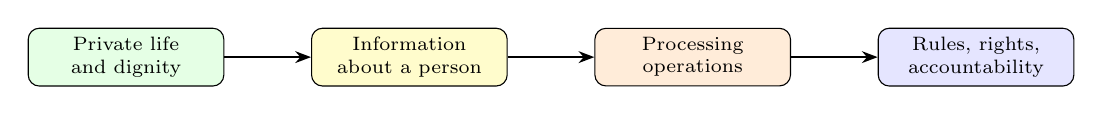
\begin{tikzpicture}[node distance=1.1cm]
\node[privacybox, fill=green!10] (private) {Private life\\and dignity};
\node[privacybox, right=of private, fill=yellow!20] (info) {Information\\about a person};
\node[privacybox, right=of info, fill=orange!15] (processing) {Processing\\operations};
\node[privacybox, right=of processing, fill=blue!10] (governance) {Rules, rights,\\accountability};
\draw[privacyarrow] (private) -- (info);
\draw[privacyarrow] (info) -- (processing);
\draw[privacyarrow] (processing) -- (governance);
\end{tikzpicture}
\end{adjustbox}
\end{center}

\begin{block}{Reading the scheme}
Privacy protects private life. Data protection adds governance for the life cycle of information.
\end{block}
\end{frame}

\takeawaysframe{
\begin{itemize}
    \item Privacy is not only secrecy; it protects autonomy and dignity.
    \item Data protection focuses on the circulation and use of personal information.
    \item Healthcare needs controlled data sharing, not total data isolation.
\end{itemize}
}{
St. Isidore must protect patients from exposure while still allowing data to move safely for care.
}

\section{Healthcare Data}
\sectiontitleframe{Healthcare Data}

\begin{frame}[c]{Section Context: Healthcare Data}
\begin{block}{What we are talking about}
Healthcare data is especially sensitive because it can affect treatment, employment, insurance,
family relations, stigma, and personal safety. Many laws treat health information as requiring
stronger protection than ordinary administrative data.
\end{block}

\begin{exampleblock}{Hospital lens}
A patient phone number is personal data. A diagnosis, HIV test, pregnancy record, genetic marker, or
mental-health note can expose intimate facts and future risks.
\end{exampleblock}
\end{frame}

\begin{frame}[c]{Personal Data and Medical Data}
\begin{block}{Distinction}
\textbf{Personal data} identifies or can identify a person. \textbf{Medical data} is generated in
care: symptoms, diagnoses, medication, tests, imaging, procedures, outcomes, and clinical notes.
\end{block}

\begin{exampleblock}{Running example}
The string ``Maria Rossi'' identifies a patient. ``Positive malaria test'', ``CD4 count'', or
``post-operative infection'' is medical data. Together, they become highly sensitive patient
information.
\end{exampleblock}
\end{frame}

\begin{frame}[c]{PHI as a Practical Teaching Term}
\begin{block}{Protected health information}
Healthcare privacy literature often uses \textbf{PHI} for information linked to a person's health
status and care. The exact legal term differs by jurisdiction, but the operational idea is stable:
health-linked identifiable data deserves enhanced safeguards \cite{conduah2025}.
\end{block}

\begin{exampleblock}{Running example}
An appointment ID alone may look harmless. If it links to oncology, psychiatry, infectious disease,
or maternity services, it can become sensitive.
\end{exampleblock}
\end{frame}

\begin{frame}[c]{Why Healthcare Data Is Hard to Protect}
\begin{block}{Practical tension}
Healthcare data must be available quickly for treatment, but it must not become freely visible to
everyone. Care delivery, billing, public health, quality control, and research all create pressure to
reuse data.
\end{block}

\begin{exampleblock}{Running example}
In emergency care, a clinician needs allergies and medication history immediately. A marketing
contractor does not need the same access to the same record.
\end{exampleblock}
\end{frame}

\begin{frame}[c]{Healthcare Data Life Cycle}
\begin{center}
\begin{adjustbox}{max width=\textwidth}
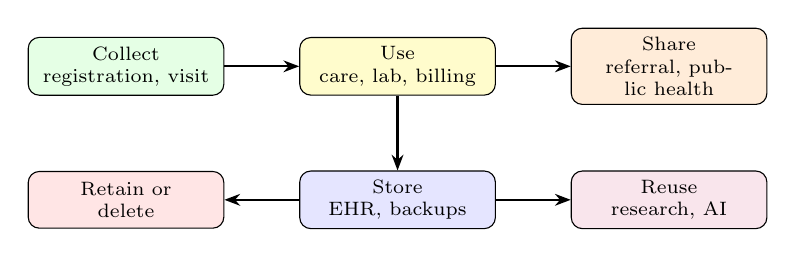
\begin{tikzpicture}[node distance=0.95cm]
\node[privacybox, fill=green!10] (collect) {Collect\\registration, visit};
\node[privacybox, right=of collect, fill=yellow!20] (use) {Use\\care, lab, billing};
\node[privacybox, right=of use, fill=orange!15] (share) {Share\\referral, public health};
\node[privacybox, below=of use, fill=blue!10] (store) {Store\\EHR, backups};
\node[privacybox, right=of store, fill=purple!10] (reuse) {Reuse\\research, AI};
\node[privacybox, left=of store, fill=red!10] (delete) {Retain or\\delete};
\draw[privacyarrow] (collect) -- (use);
\draw[privacyarrow] (use) -- (share);
\draw[privacyarrow] (use) -- (store);
\draw[privacyarrow] (store) -- (reuse);
\draw[privacyarrow] (store) -- (delete);
\end{tikzpicture}
\end{adjustbox}
\end{center}
\end{frame}

\takeawaysframe{
\begin{itemize}
    \item Health data can identify, stigmatize, and harm patients.
    \item Sensitivity often comes from context and linkage, not only from one field.
    \item Privacy controls must follow the whole data life cycle.
\end{itemize}
}{
St. Isidore must ask not only ``who can open the EHR?'' but also ``where does the data go next?''
}

\section{Global Frameworks}
\sectiontitleframe{Global Frameworks}

\begin{frame}[c]{Section Context: Global Frameworks}
\begin{block}{What we are talking about}
Data protection rules differ across countries, but many share a family resemblance: lawful
collection, purpose limitation, data quality, security, individual rights, accountability, and rules
for cross-border flows.
\end{block}

\begin{exampleblock}{Hospital lens}
A patient may be treated locally, tested by an external laboratory, followed through a cloud
telemedicine platform, and included in international research. Privacy rules must travel with that
workflow.
\end{exampleblock}
\end{frame}

\begin{frame}[c]{International Building Blocks}
\begin{block}{Common roots}
The Universal Declaration of Human Rights, the European Convention on Human Rights, Council of
Europe Convention 108, and OECD Privacy Guidelines helped shape modern privacy and data protection
thinking \cite{udhr,echr,coe108,oecd_privacy}.
\end{block}

\begin{exampleblock}{Running example}
Even before choosing a specific law, \scenario{} can recognize baseline principles: avoid arbitrary
interference, define purposes, limit collection, protect security, and allow people some control.
\end{exampleblock}
\end{frame}

\begin{frame}[c]{Why GDPR Became a Reference Model}
\begin{block}{Global influence}
GDPR combined broad territorial reach, strong rights, accountability, security duties, independent
supervision, and cross-border transfer rules. Its structure has influenced policy debates and many
regulatory reforms, even outside Europe \cite{eurlex_gdpr,eu_framework}.
\end{block}

\begin{exampleblock}{Careful wording}
GDPR is not copied everywhere. Some systems focus on sectors, consumers, constitutional privacy,
public health, or cyber duties. It is best treated as a mature reference architecture, not as a
universal template.
\end{exampleblock}
\end{frame}

\begin{frame}[c]{Healthcare Privacy Across Regions}
\small
\begin{tabularx}{\textwidth}{@{}p{0.19\textwidth}p{0.24\textwidth}X@{}}
\toprule
\textbf{Framework} & \textbf{Typical focus} & \textbf{Healthcare lesson} \\
\midrule
GDPR & general data protection & health data needs strong legal basis and safeguards \\
HIPAA & US health sector & sector-specific privacy, security, and breach rules for ePHI \\
CCPA/CPRA & consumer privacy & patient data may also appear in consumer digital services \\
POPIA & South Africa & comprehensive protection with regional implementation challenges \\
APEC & cross-border privacy & interoperability matters for data flows \\
\bottomrule
\end{tabularx}
\end{frame}

\begin{frame}[c]{Regulatory Fragmentation}
\begin{block}{Problem}
Global healthcare privacy is difficult because definitions, enforcement capacity, security
expectations, breach reporting, consent rules, and infrastructure differ across jurisdictions
\cite{conduah2025}.
\end{block}

\begin{exampleblock}{Running example}
If St. Isidore joins a multicountry malaria study, one partner may require ethics approval and
pseudonymization, another may require local storage, and a cloud tool may trigger transfer rules.
\end{exampleblock}
\end{frame}

\takeawaysframe{
\begin{itemize}
    \item GDPR is a strong reference example, not the only privacy law.
    \item Many regimes share principles, but implementation differs.
    \item Cross-border healthcare workflows need legal and technical interoperability.
\end{itemize}
}{
St. Isidore cannot solve privacy by naming one law; it must map data flows and applicable duties.
}

\section{GDPR Concepts}
\sectiontitleframe{GDPR Concepts}

\begin{frame}[c]{Section Context: GDPR Concepts}
\begin{block}{What we are talking about}
GDPR gives vocabulary that is useful beyond Europe: personal data, processing, data subject,
controller, processor, principles, legal basis, special categories, rights, and accountability.
\end{block}

\begin{exampleblock}{Hospital lens}
These words help translate a messy hospital workflow into governance questions: who decides, who
acts, why data is used, how much is needed, and how patients can exercise control.
\end{exampleblock}
\end{frame}

\begin{frame}[c]{Personal Data and Identifiability}
\begin{block}{Core idea}
Personal data is any information relating to an identified or identifiable natural person. A person
may be identified directly, or indirectly through identifiers, location, online IDs, or physical,
genetic, economic, cultural, social, or other characteristics \cite{eurlex_gdpr}.
\end{block}

\begin{exampleblock}{Running example}
``Patient 1042'' may still be personal data if the hospital can link that number to a name. A rare
disease plus village plus admission date may also identify someone indirectly.
\end{exampleblock}
\end{frame}

\begin{frame}[c]{The Identifiability Test}
\begin{block}{Reasonable means}
Identifiability depends on what the controller or another party can reasonably use, considering
cost, time, available technology, and likely future developments.
\end{block}

\begin{exampleblock}{Running example}
A dataset with ages, postal codes, rare diagnoses, and dates may look anonymous. If local staff can
match it with appointment schedules, it may still identify patients.
\end{exampleblock}
\end{frame}

\begin{frame}[c]{Anonymization vs Pseudonymization}
\begin{block}{Different risk levels}
\textbf{Anonymization} aims to make re-identification no longer reasonably possible.
\textbf{Pseudonymization} replaces direct identifiers with codes, but someone can still re-link the
data using additional information.
\end{block}

\begin{exampleblock}{Running example}
Removing names from lab results is not enough if a separate key links code \texttt{P-1042} to Maria.
That is pseudonymized data, not anonymous data.
\end{exampleblock}
\end{frame}

\begin{frame}[c]{Processing Means Almost Everything}
\begin{block}{Processing}
Processing includes collecting, recording, organizing, storing, changing, consulting, using,
transmitting, making available, comparing, linking, restricting, erasing, and destroying data.
\end{block}

\begin{exampleblock}{Running example}
When a nurse opens a record, a lab uploads a result, a backup stores the database, or a research
team receives an export, each action is processing.
\end{exampleblock}
\end{frame}

\begin{frame}[c]{Actors in a Data Processing Workflow}
\begin{center}
\begin{adjustbox}{max width=\textwidth}
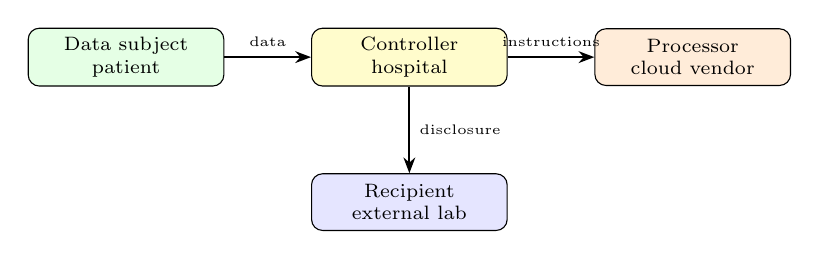
\begin{tikzpicture}[node distance=1.1cm]
\node[privacybox, fill=green!10] (subject) {Data subject\\patient};
\node[privacybox, right=of subject, fill=yellow!20] (controller) {Controller\\hospital};
\node[privacybox, right=of controller, fill=orange!15] (processor) {Processor\\cloud vendor};
\node[privacybox, below=of controller, fill=blue!10] (recipient) {Recipient\\external lab};
\draw[privacyarrow] (subject) -- node[above,font=\tiny]{data} (controller);
\draw[privacyarrow] (controller) -- node[above,font=\tiny]{instructions} (processor);
\draw[privacyarrow] (controller) -- node[right,font=\tiny]{disclosure} (recipient);
\end{tikzpicture}
\end{adjustbox}
\end{center}
\end{frame}

\begin{frame}[c]{Controller and Processor}
\begin{block}{Responsibility structure}
The \textbf{controller} determines purposes and means. The \textbf{processor} processes personal data
on behalf of the controller. Joint controllers may exist when multiple parties jointly decide why and
how processing happens.
\end{block}

\begin{exampleblock}{Running example}
\scenario{} decides to use an EHR for patient care: it is the controller. A hosting provider that
runs the database under hospital instructions is usually a processor.
\end{exampleblock}
\end{frame}

\begin{frame}[c]{GDPR Object, Scope, and Balance}
\begin{block}{Object}
GDPR protects natural persons with regard to personal-data processing and also supports free
movement of personal data within the EU. It balances data protection, legitimate data flows, and
other rights such as information, research, and non-discrimination.
\end{block}

\begin{exampleblock}{Running example}
A hospital should not block every data transfer in the name of privacy. It should allow necessary
care, public health, and research flows under defined safeguards.
\end{exampleblock}
\end{frame}

\takeawaysframe{
\begin{itemize}
    \item Personal data depends on identifiability, including indirect identifiability.
    \item Pseudonymized data can still be personal data.
    \item Governance starts by naming actors, purposes, and processing operations.
\end{itemize}
}{
St. Isidore can now describe a patient-data workflow before deciding whether it is lawful or safe.
}

\section{Principles and Legal Bases}
\sectiontitleframe{Principles and Legal Bases}

\begin{frame}[c]{Section Context: Principles and Legal Bases}
\begin{block}{What we are talking about}
Modern data protection law does not only ask whether data is secret. It asks whether processing is
lawful, fair, transparent, purpose-bound, minimized, accurate, time-limited, secure, and
demonstrably governed.
\end{block}

\begin{exampleblock}{Hospital lens}
The same patient record may be lawful for treatment, unlawful for curiosity, and risky for research
unless it is governed by an appropriate legal basis and safeguards.
\end{exampleblock}
\end{frame}

\begin{frame}[c]{Principles of Processing}
\small
\begin{tabularx}{\textwidth}{@{}p{0.28\textwidth}X@{}}
\toprule
\textbf{Principle} & \textbf{Hospital question} \\
\midrule
Lawfulness, fairness, transparency & Why can we use this data, and has the patient been informed? \\
Purpose limitation & What exact care, billing, research, or public-health purpose? \\
Data minimization & Which fields are necessary? \\
Accuracy & Is the allergy, diagnosis, or contact data correct? \\
Storage limitation & How long do we keep it? \\
Integrity and confidentiality & Who can access it, and how is it secured? \\
Accountability & Can we prove our controls and decisions? \\
\bottomrule
\end{tabularx}
\end{frame}

\begin{frame}[c]{Legal Bases: Consent Is Only One Option}
\begin{block}{Lawfulness}
GDPR lists several legal bases: consent, contract, legal obligation, vital interests, public task,
and legitimate interests. Healthcare often relies on legal obligation, public interest, vital
interests, or healthcare-specific grounds, not only consent.
\end{block}

\begin{exampleblock}{Running example}
An unconscious patient cannot meaningfully consent in the emergency room. Treatment may still be
necessary to protect vital interests and deliver care under health-system rules.
\end{exampleblock}
\end{frame}

\begin{frame}[c]{Consent: Strong but Fragile}
\begin{block}{Elements}
Consent must be freely given, specific, informed, and unambiguous. For sensitive data, explicit
consent may be required in some contexts, but health law may also provide other grounds.
\end{block}

\begin{exampleblock}{Running example}
``Accept all hospital data uses'' is not specific. Separate choices may be needed for appointment
reminders, research contact, patient portal analytics, or optional wellness programs.
\end{exampleblock}
\end{frame}

\begin{frame}[c]{Why Online Consent Often Fails}
\begin{block}{Practical weakness}
Online consent may be bundled, manipulated by interface design, poorly understood, hard to refuse,
or harder to withdraw than to give. Notice-and-consent alone is weak when patients face power
imbalances or urgent care needs.
\end{block}

\begin{exampleblock}{Running example}
A patient should not be forced to accept marketing analytics in order to book an essential oncology
appointment.
\end{exampleblock}
\end{frame}

\begin{frame}[c]{Special Categories: Health Data}
\begin{block}{Higher protection}
Data revealing health, genetics, biometrics used for unique identification, sex life, or other
special categories is generally subject to a prohibition unless a specific exception applies.
\end{block}

\begin{exampleblock}{Running example}
The hospital may process blood-test results for care, but reuse for AI product development needs a
separate legal and ethical analysis.
\end{exampleblock}
\end{frame}

\takeawaysframe{
\begin{itemize}
    \item Principles turn privacy into operational design questions.
    \item Consent is important, but healthcare cannot be reduced to consent banners.
    \item Health data usually needs stronger safeguards and clearer justification.
\end{itemize}
}{
St. Isidore must document why each data use exists and why the chosen data is necessary.
}

\section{Rights of Patients}
\sectiontitleframe{Rights of Patients}

\begin{frame}[c]{Section Context: Rights of Patients}
\begin{block}{What we are talking about}
Data protection gives people enforceable rights over information about them. In healthcare, those
rights must be handled carefully because records also support safety, continuity of care, legal
retention, and professional accountability.
\end{block}

\begin{exampleblock}{Hospital lens}
A patient asking for a copy of their record is not making an IT request. They are exercising control
over information that may shape future care and personal life.
\end{exampleblock}
\end{frame}

\begin{frame}[c]{Core Rights}
\small
\begin{tabularx}{\textwidth}{@{}p{0.24\textwidth}X@{}}
\toprule
\textbf{Right} & \textbf{Hospital meaning} \\
\midrule
Information & clear privacy notice and explanation of purposes \\
Access & know whether data is processed and obtain relevant information \\
Rectification & correct inaccurate data and complete incomplete data \\
Erasure & delete data when grounds apply, subject to limits \\
Restriction & pause certain processing while issues are resolved \\
Portability & receive and transfer data in structured format where applicable \\
Objection & object to certain public-task or legitimate-interest processing \\
Automated decisions & protections against solely automated significant decisions \\
\bottomrule
\end{tabularx}
\end{frame}

\begin{frame}[c]{Information and Access}
\begin{block}{Transparency in practice}
Patients should know who processes data, for which purposes, on what legal basis, who receives it,
how long it is kept, whether automated decisions exist, and how to exercise rights.
\end{block}

\begin{exampleblock}{Running example}
If \scenario{} sends samples to an external laboratory, the privacy notice should not hide that
relationship behind vague wording such as ``trusted partners''.
\end{exampleblock}
\end{frame}

\begin{frame}[c]{Rectification and Clinical Safety}
\begin{block}{Accuracy matters}
The right to rectification reflects the principle of accuracy. In healthcare, wrong data can cause
direct physical harm, not only privacy harm.
\end{block}

\begin{exampleblock}{Running example}
If the EHR wrongly records that a patient has no penicillin allergy, rectification is a safety
control. If it records the wrong phone number, confidentiality can also fail.
\end{exampleblock}
\end{frame}

\begin{frame}[c]{Erasure and Its Limits}
\begin{block}{Not a simple delete button}
Erasure may apply when data is no longer necessary, consent is withdrawn and no other basis exists,
or processing is unlawful. But healthcare records may also be subject to legal retention, medical
liability, public-health, or patient-safety duties.
\end{block}

\begin{exampleblock}{Running example}
A patient may ask to delete marketing preferences. Deleting a surgical record needed for continuity
of care is a different question.
\end{exampleblock}
\end{frame}

\begin{frame}[c]{Automated Decisions and Profiling}
\begin{block}{High-stakes automation}
Profiling uses personal data to evaluate or predict aspects of a person, including health,
behavior, reliability, or location. Solely automated decisions with significant effects require
special safeguards.
\end{block}

\begin{exampleblock}{Running example}
An AI triage tool may support a clinician. A fully automated refusal of specialist referral based on
a risk score would require close legal, ethical, and clinical scrutiny.
\end{exampleblock}
\end{frame}

\takeawaysframe{
\begin{itemize}
    \item Rights make privacy operational for patients.
    \item Healthcare rights must be balanced with safety and lawful retention.
    \item Automated systems need transparency, human oversight, and contestability.
\end{itemize}
}{
St. Isidore needs workflows for rights requests, not just a privacy policy page.
}

\section{Accountability and Design}
\sectiontitleframe{Accountability and Design}

\begin{frame}[c]{Section Context: Accountability and Design}
\begin{block}{What we are talking about}
GDPR's philosophy is accountability: the controller must choose appropriate technical and
organizational measures and be able to prove them. Compliance is not only paperwork; it is design,
operation, monitoring, and review.
\end{block}

\begin{exampleblock}{Hospital lens}
If a breach occurs, \scenario{} must explain what data was processed, why, who had access, which
controls existed, how risks were assessed, and what changed after the incident.
\end{exampleblock}
\end{frame}

\begin{frame}[c]{Accountability Architecture}
\begin{center}
\begin{adjustbox}{max width=\textwidth}
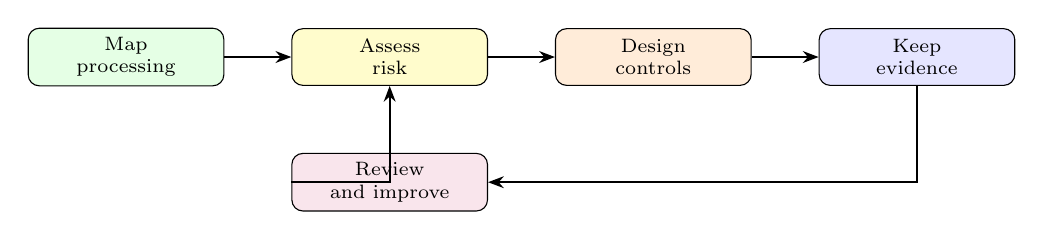
\begin{tikzpicture}[node distance=0.85cm]
\node[privacybox, fill=green!10] (map) {Map\\processing};
\node[privacybox, right=of map, fill=yellow!20] (risk) {Assess\\risk};
\node[privacybox, right=of risk, fill=orange!15] (controls) {Design\\controls};
\node[privacybox, right=of controls, fill=blue!10] (evidence) {Keep\\evidence};
\node[privacybox, below=of risk, fill=purple!10] (review) {Review\\and improve};
\draw[privacyarrow] (map) -- (risk);
\draw[privacyarrow] (risk) -- (controls);
\draw[privacyarrow] (controls) -- (evidence);
\draw[privacyarrow] (evidence) |- (review);
\draw[privacyarrow] (review.west) -| (risk.south);
\end{tikzpicture}
\end{adjustbox}
\end{center}
\end{frame}

\begin{frame}[c]{Data Protection by Design and by Default}
\begin{block}{Design rule}
Privacy must be built into systems when purposes and means are chosen, and during processing.
Default settings should process only the data necessary for each purpose, with limited access,
scope, retention, and visibility.
\end{block}

\begin{exampleblock}{Running example}
The laboratory dashboard should default to lab requests and results, not the full psychiatric and
billing history of every patient.
\end{exampleblock}
\end{frame}

\begin{frame}[c]{Technical and Organizational Measures}
\small
\begin{tabularx}{\textwidth}{@{}p{0.28\textwidth}X@{}}
\toprule
\textbf{Measure} & \textbf{Healthcare example} \\
\midrule
Access control & roles for clinicians, lab, admin, researcher \\
Encryption & protect laptops, backups, APIs, and data transfers \\
Pseudonymization & research exports separated from direct identifiers \\
Logging and audit & detect unusual access to celebrity or staff records \\
Retention rules & keep records as required, delete optional data sooner \\
Training and policy & staff know when sharing is legitimate \\
Vendor governance & processor contracts and security requirements \\
\bottomrule
\end{tabularx}
\end{frame}

\begin{frame}[c]{Breach Notification and DPIA}
\begin{block}{Risk-triggered duties}
Some obligations depend on risk: personal-data breaches may require notification to a supervisory
authority and, in higher-risk cases, communication to affected people. High-risk processing may
require a Data Protection Impact Assessment.
\end{block}

\begin{exampleblock}{Running example}
A lost encrypted laptop may be low risk if keys are safe. A leaked spreadsheet of identifiable HIV
results is high risk and demands urgent legal, technical, and patient-support action.
\end{exampleblock}
\end{frame}

\begin{frame}[c]{DPO and Supervisory Authorities}
\begin{block}{Oversight}
Modern data protection often includes independent supervisory authorities and, in some
organizations, a Data Protection Officer. Their role is to help ensure that privacy duties are not
left to ad hoc technical judgment alone.
\end{block}

\begin{exampleblock}{Running example}
When \scenario{} plans an AI triage pilot, the DPO, clinicians, security team, and ethics board
should be involved before deployment.
\end{exampleblock}
\end{frame}

\takeawaysframe{
\begin{itemize}
    \item Accountability means choosing controls and proving they work.
    \item By design and by default connects privacy to system architecture.
    \item Breach response and DPIA are risk-management tools.
\end{itemize}
}{
St. Isidore turns privacy from a document into a repeatable governance process.
}

\section{Privacy Risks in Digital Healthcare}
\sectiontitleframe{Privacy Risks in Digital Healthcare}

\begin{frame}[c]{Section Context: Digital Healthcare Risks}
\begin{block}{What we are talking about}
Electronic records, cloud services, APIs, analytics, mobile apps, and AI increase both care value
and privacy risk. Security failures, poor governance, and unclear data flows can all undermine
patient trust.
\end{block}

\begin{exampleblock}{Hospital lens}
The same API that helps the emergency department retrieve records quickly can also expose large
volumes of patient data if authentication, authorization, logging, or contracts fail.
\end{exampleblock}
\end{frame}

\begin{frame}[c]{Breach Examples}
\begin{block}{What major incidents teach}
Large healthcare breaches and disruptions, including Anthem, WannaCry/NHS, SingHealth, and other
regional incidents, show that legal frameworks alone cannot protect data without resilient systems,
patching, segmentation, backups, monitoring, and governance \cite{conduah2025}.
\end{block}

\begin{exampleblock}{Running example}
If ransomware blocks laboratory results, privacy, safety, and availability fail together. Patients
are harmed even if no one reads the data.
\end{exampleblock}
\end{frame}

\begin{frame}[c]{Privacy, Security, and Trust}
\begin{block}{Relationship}
Security is not identical to privacy, but privacy depends on security. Confidentiality, integrity,
and availability protect patient data so that information is not exposed, corrupted, or unavailable
when care depends on it.
\end{block}

\begin{exampleblock}{Running example}
Encryption protects confidentiality. Audit logs support accountability. Backups protect
availability. All three contribute to patient trust.
\end{exampleblock}
\end{frame}

\begin{frame}[c]{Technology Helps, but Does Not Replace Governance}
\begin{block}{Emerging tools}
AI and machine learning can support anomaly detection, risk prediction, and compliance monitoring.
Blockchain can support integrity and traceability in some sharing scenarios. But tools can also
create new data flows, inference risks, and accountability questions.
\end{block}

\begin{exampleblock}{Running example}
An AI model that detects unusual EHR access is useful. An AI model trained on excessive patient
details without a valid purpose creates a new privacy problem.
\end{exampleblock}
\end{frame}

\begin{frame}[c]{From Previous Lessons to Privacy}
\small
\begin{tabularx}{\textwidth}{@{}p{0.26\textwidth}X@{}}
\toprule
\textbf{Previous topic} & \textbf{Privacy connection} \\
\midrule
Networking & segment systems so not every subnet can reach every API \\
Authentication & know who is accessing patient data \\
Access control & limit users to legitimate roles and tasks \\
Encryption & protect data at rest and in transit \\
Logging & produce evidence of access, changes, and incidents \\
\bottomrule
\end{tabularx}
\end{frame}

\takeawaysframe{
\begin{itemize}
    \item Digital healthcare privacy is legal, ethical, and technical.
    \item Breaches show that compliance language is not enough.
    \item Security controls become privacy safeguards when tied to purpose and rights.
\end{itemize}
}{
St. Isidore's earlier security controls now become part of patient-data protection.
}

\section{Final Integration}
\sectiontitleframe{Final Integration}

\begin{frame}[c]{Final Concept Map}
\begin{center}
\begin{adjustbox}{max width=\textwidth}
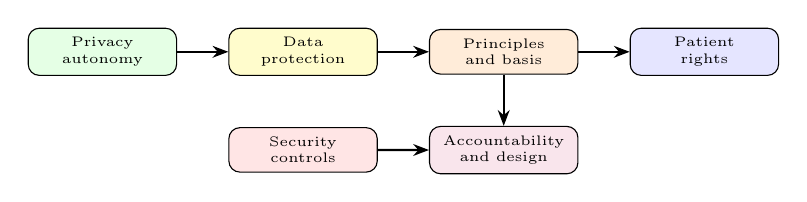
\begin{tikzpicture}[node distance=0.65cm]
\node[smallprivacybox, fill=green!10] (privacy) {Privacy\\autonomy};
\node[smallprivacybox, right=of privacy, fill=yellow!20] (data) {Data\\protection};
\node[smallprivacybox, right=of data, fill=orange!15] (principles) {Principles\\and basis};
\node[smallprivacybox, right=of principles, fill=blue!10] (rights) {Patient\\rights};
\node[smallprivacybox, below=of principles, fill=purple!10] (account) {Accountability\\and design};
\node[smallprivacybox, below=of data, fill=red!10] (security) {Security\\controls};
\draw[privacyarrow] (privacy) -- (data);
\draw[privacyarrow] (data) -- (principles);
\draw[privacyarrow] (principles) -- (rights);
\draw[privacyarrow] (principles) -- (account);
\draw[privacyarrow] (security) -- (account);
\end{tikzpicture}
\end{adjustbox}
\end{center}
\end{frame}

\begin{frame}[c]{Final Recap}
\begin{block}{Core lesson}
Healthcare privacy is not only confidentiality. It is the governance of identifiable health data
throughout its life cycle: lawful purpose, minimal use, transparency, patient rights, security,
accountability, and evidence.
\end{block}

\begin{exampleblock}{In \scenario}
St. Isidore can use EHRs, APIs, labs, research datasets, and AI tools, but each data flow must have
a reason, a limit, a safeguard, and someone accountable for it.
\end{exampleblock}
\end{frame}

\begin{frame}[allowframebreaks]{References}
\bibliographystyle{apalike-AMS}
\bibliography{main}
\end{frame}

\end{document}
